\section{Requirements}

\subsection{Project Organisation}
This project is a part of a larger project investigating the effect of using high-radix number representation with online arithmetic operators.
The overarching aim involves implementing such a system on an FPGA and quantifying its performance improvements.
This is achieved through two individual projects, vertically split from the enveloping project.
One shall design the arithmetic operator modules, while the other shall design a system from the top-level to test and evaluate these operators.
This project deals with the system-level issues.

As this project progresses in parallel with the designing of the operator modules, it is necessary to decouple the two projects so that, being individual projects, they can be evaluated individually.
The success of one project should not be restricted by the status of the other.
To this end, the goal of the system-level design is more focussed on its functionalities and robustness.
This relationship and its effect on the evaluation will be examined further in the evaluation chapter of this report.

To ensure the two products will work together once they are both complete, a common interface is agreed upon.
The interface will be done using Qsys.
The unit-level project will build different operators, which can have varying arithmetic functions and designs.
These can be packaged into individual Qsys modules, as adders, multipliers, or dividers.
Alternatively they can also be delivered as a single module taking two operands and an instruction that is one of the four basic arithmetic operations.
These will then become the DUTs of the testbench.

\subsection{Deliverables}
At the end of the project, the system should be able to perform the following:
\begin{enumerate}
  \item Connect to the arithmetic modules as its input;
  \item Generate and run tests on these modules;
  \item Vary the frequency of the FPGA;
  \item Evaluate its performance.
\end{enumerate}

\subsection{Hardware Choice}
The system itself will be built on a Cyclone V SX SoC Development Board from Intel~\cite{Intel1}.

\begin{figure}[H]
  \centering
  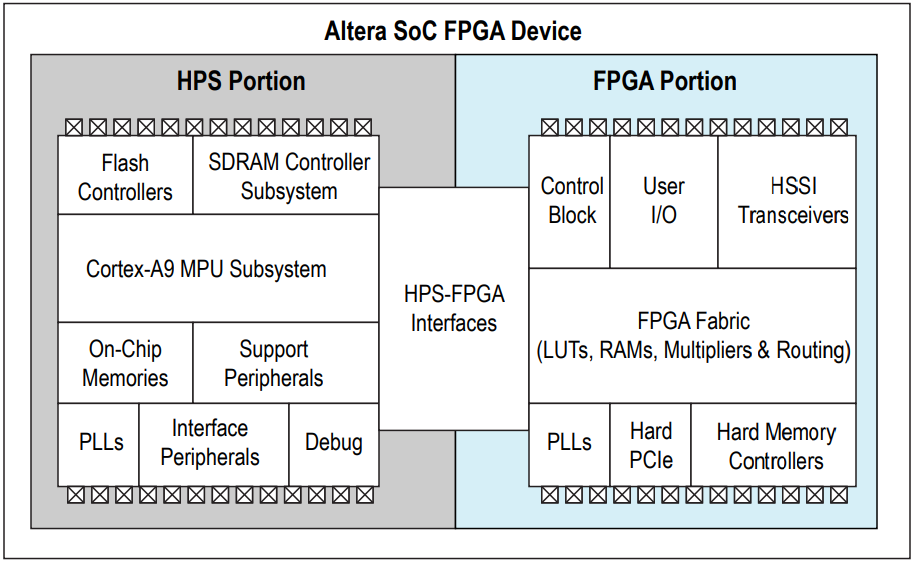
\includegraphics[width=10cm]{img/SoCStructure}
  \caption{Structure of the System-on-Chip}
  \label{SoCStructure}
\end{figure}

The 5CSXFC6D6F31C6N SoC has an Arm Cortex-A9 MPCore accompanied by Intel's 28nm FPGA fabric~\cite{Altera1}.
The FPGA is necessary for implementing the hardware design and obtaining empirical results for the project.
% maybe hybrid architecture soc makes programming it harder and it could % be used as a negative point 
While an FPGA without an embedded CPU will be enough for this project to work, having an Hard Processor System (HPS) on the same chip is useful as the test software can run on it.
The HPS is a separate piece of hardware that distinguishes itself from a soft processor, such as the Nios II, a processor programmed onto the FPGA itself.
With this additional capacity, a better user interface can thus be constructed with more detailed, on-the-fly control of the FPGA.
This means setting up the testbench will only require programming the design into the FPGA, followed by running the test script on the HPS.
The product will thus be self-contained.
It will be more accessible as no additional setup is required for the user.

It should be noted that Xilinx offers similar boards as well.
Its Zynq SoC family has a very comparable structure as they too integrate the software programmability of an Arm processor with the hardware possibility of an FPGA.
For example, similar to the Cyclone V SX, Zynq-7000S features an Arm Cortex-A9
coupled with a Xilinx 28nm FPGA~\cite{Xilinx1}.
As such, a board like the ZedBoard~\cite{Xilinx2} could be just as viable for this project.

As there are very few significant functional differences between the two brands, I shall initially explore with the Intel board, simply for its availability and my familiarity with their development tools.
Due to the architectural differences between the logic elements between Xilinx and Altera FPGAs~\cite{Scekic1}, the performances on the two boards are not necessarily identical.
Once the project has progressed to a point where the system design is mature and tested, the Xilinx alternative can be explored as an extension.

\subsection{Software Choice}
The software choice follows closely with the hardware choice in this project.
To develop for Intel FPGAs, Quartus has to be used.
The version picked is arbitrary as there are not many functional differences between the versions that will be critical to the project.
As Quartus Prime 16.0 is the version installed in the computers in the department, I will use the same version simply for convenience.
This naturally means the hardware system will be built with the system integration tool that comes with Quartus -- Qsys.

The Qsys software is designed to be used for integrating different hardware modules into a system.
As such, it will be used as the interface for the two parallel projects.

While an HLS language could be used, in this design it suffers from a few problems and does not offer enough benefits to justify its use.
Usually HLS is preferred for developing complex algorithms, because compilers can optimise them into RTL much better than humans.
However, the resulting RTL would be unreadable, making directly controlling or debugging at the hardware level nearly impossible.
The interfaces require detailed control of the actual hardware and the rest of the testbench has a lot of control path work and direct manipulation on the data bits.
It is therefore not worth it to use HLS and as such, this design will be written in Verilog.

Other than the hardware design tools, there is some freedom of choice on the HPS side of the project.
The test will be built with Python, which will be running on an Ubuntu system that is installed on the HPS.
This choice is made as there are previous unrelated projects on the same development board, which means a lot of time can be saved on tedious setup works such as getting an operating system booting.

Git is used as the version control system for this project.
A list of repositories on GitHub holds all files related to this project.
Readme files on the repositories and the commit histories will serve as digital logbooks to this project.
